\section{\acf{CPS}}
\acf{CPS} refer to a network of distributed controllers that are used to control adjoining physical processes~\cite{alur2015principles}~\cite{CPSDesignChallenges}. 
\ac{CPS} encompass a wide variety of disciplines, from mechatronics to civil infrastructure (Figure~\ref{fig:cps}).
\ac{CPS} operate in the physical world, where environments can be unpredictable and uncontrollable.
\ac{CPS} applications encompass real-time systems, where the systems need to satisfy a set of timing and functional requirements to ensure correct operation. 
Here, a missed deadline may result in catastrophic consequences, making these \ac{CPS} highly \textit{safety-critical}. 
These have strict timing and functionality requirements --- any errors in control can result in physical damage, injuries, and/or fatalities~\cite{ANNDevModel1999}. 
Hence, the hardware and software processes used in \ac{CPS} must operate in a predictable and reliable~\cite{reliable-cps}~\cite{seshia2016towards} manner at all times.
This introduces safety concerns for the \ac{CPS}.
This thesis focuses on ensuring such requirements for \ac{CPS}, especially where \acf{AI} are concerned.

\begin{figure}[h]
	\centering
	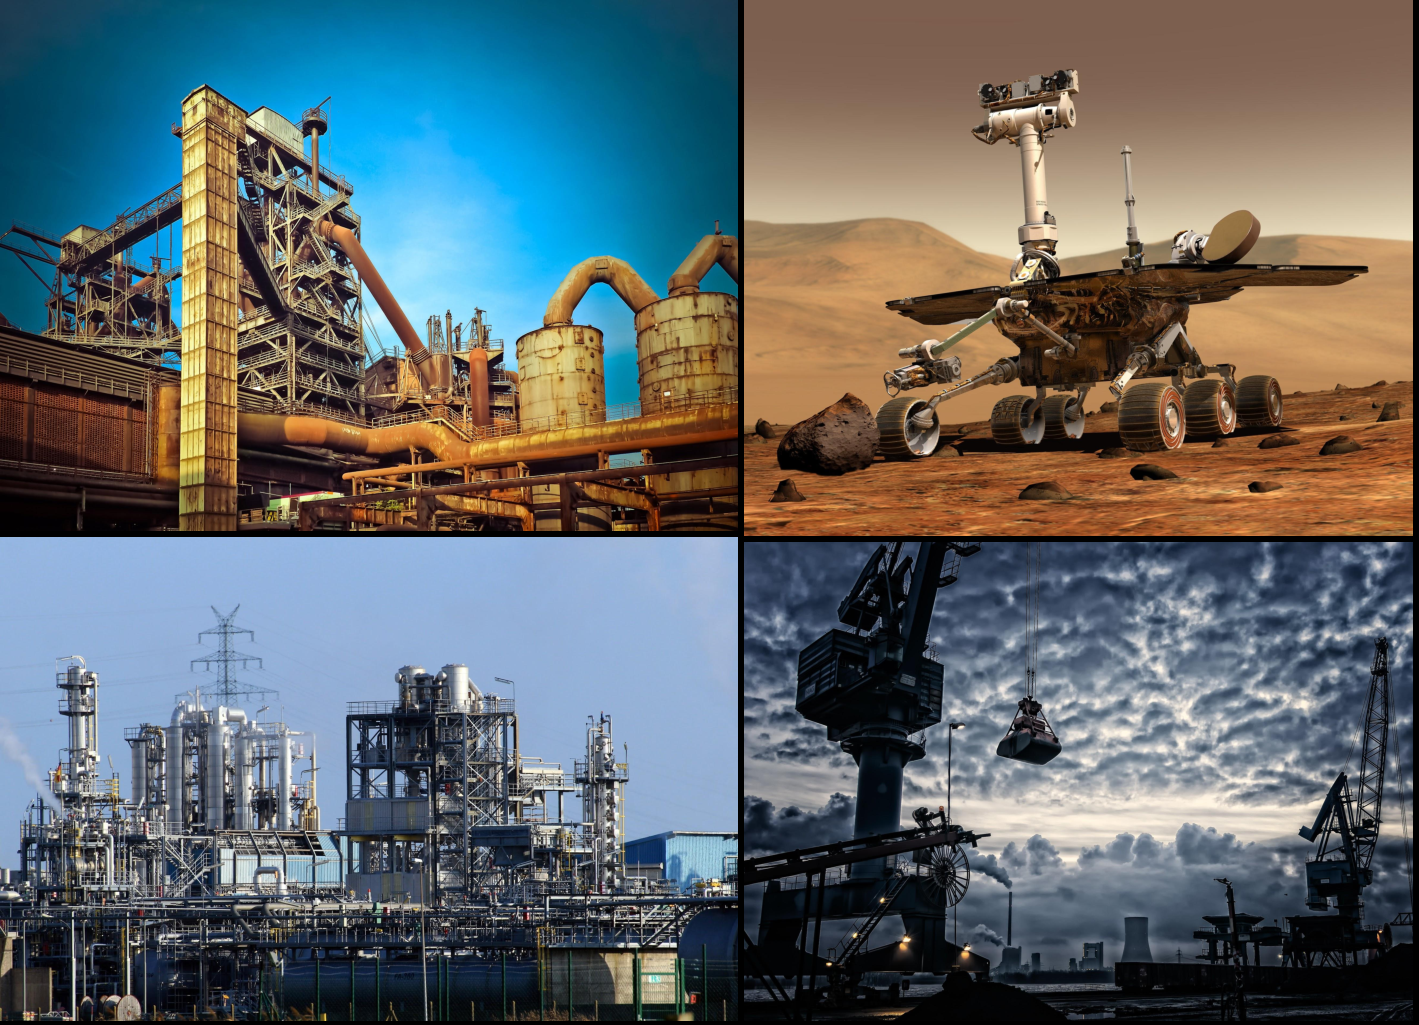
\includegraphics[width=\textwidth]{Content/fig/1234.pdf}
	\caption{Examples of \ac{CPS}~\cite{industry-pic}~\cite{crane-pic}~\cite{rover-pic}~\cite{factory-pic}, from left to right, top to bottom: A) factories, B) robotics, C) power and electricity, and D) construction \label{fig:cps}}
\end{figure}

\section{\acf{AI} and \acf{ML}}
\acf{ML} is a field of data science where \acf{AI} modules are taught to learn large and/or complex data relationships~\cite{ai}.
\ac{AI} come in many shapes and forms, from decision trees to \acfp{ANN}~\cite{ai-types}.
\ac{AI} was invented to fill a gap that humans cannot, where they can store a huge number of data relationships and learn new relationships where a human would struggle.
\ac{AI} is used all over industry, from industrial systems, to cybernetics and robotics (such as Figure~\ref{fig:ai-girl}).

\begin{figure}[h]
	\centering
	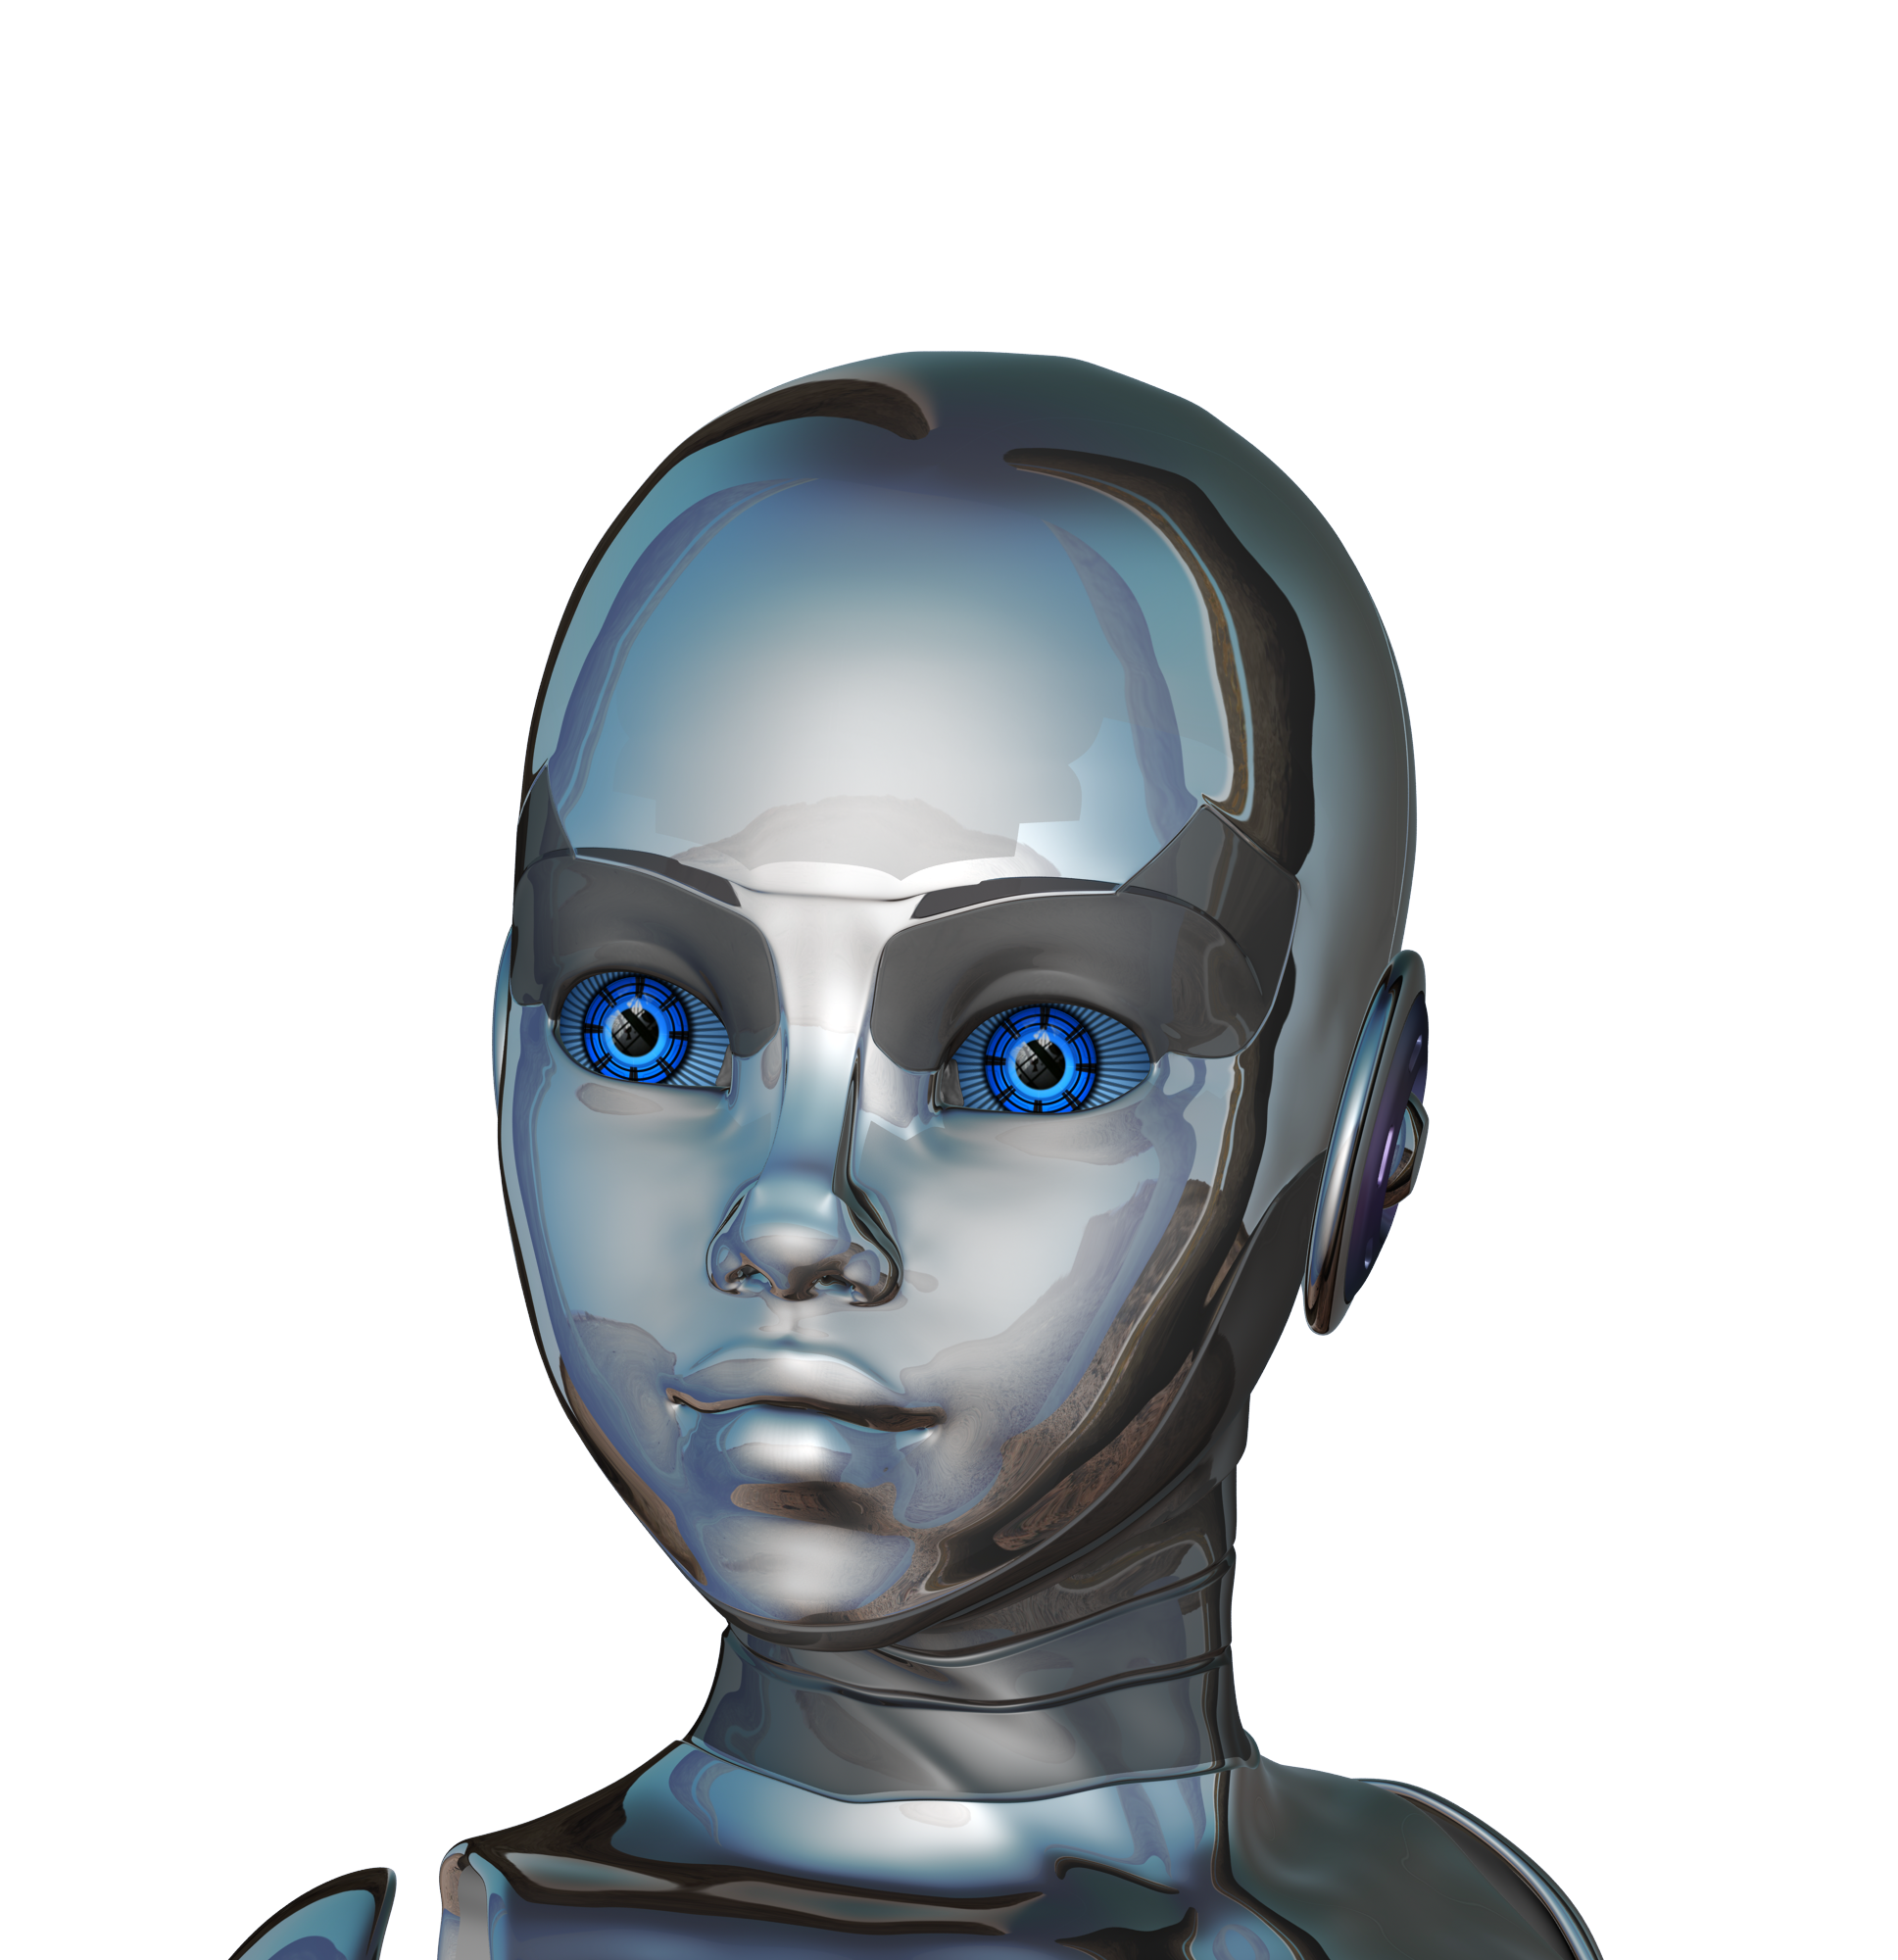
\includegraphics[width=0.4\textwidth]{Content/fig/ai-girl.png}
	\caption{\acp{AI} are frequently used as the controllers of robots~\cite{robotgirl-pic} \label{fig:ai-girl}}
\end{figure}

\ac{AI} is increasingly used in \ac{CPS}, where safety is critical.
However, the mathematical nature of \ac{AI} is non-linear, leaving many \ac{AI} applications difficult to verify.
Additionally, as \ac{AI} adapt to learn larger data sets and more complex relationships, the size and complexity of the systems increase to unmanageable proportions.
While of these are easier to verify than others~\cite{aiverify}, as they grow in size, these techniques take more time and resources to implement.
In \ac{CPS}, it is essential for all components to be verified and validated, and thus the issue with \ac{AI} in \ac{CPS} is made clear: conventional techniques cannot be used to verify \acp{AI} for \ac{CPS}.

The use of \ac{AI}, notably the \acp{ANN} used in this work, in \ac{CPS} is highly contended, as \acp{ANN} are not 100\% reliable and this can result in fatal accidents, as reported in~\cite{coldewey_2018}.
Thus, it is of utmost importance that any \ac{ANN} used in \ac{CPS} is verified to be safe for that system in all possible environments.
Without that guarantee of safety the use of \ac{AI} in such systems may pose undesirable risks~\cite{ANNSafety2018}.

Static verification methods do not carry over well to many types of \ac{AI}, including \acp{ANN}.
While some research groups can demonstrate successful functional verification methods~\cite{Gehr2018AI2SA}~\cite{reluplex}, these are often limited by the type and size of the \ac{ANN} to be verified; and the timing verification of \acp{ANN} has received scant attention.

The increase in research of \ac{AI} is causing a convergence of conventional, model-driven approaches to verification and newer, data-driven approaches~\cite{dmd2019}.
The integration of these two approaches is required using novel techniques.
The problem posed is this: how can \acp{ANN}, implemented in the model-driven design of \acp{CPS} and trained using data-driven techniques, be verified as \textit{safe}?

This thesis answers that question by introducing model-driven~\cite{dmd2019} \acfp{SNN} using the synchronous language Esterel.
Timing analysis of these \acp{SNN} is done using \acf{WCET}~\cite{wang2017timing} analysis.
Static verification techniques do not scale well with the size of system.
We address the functional safety of these \acp{SNN} using the dynamic verification techniques of \acf{RE} and \acf{RV} that do scale with the size of the system, as the system is observed as a black box during run-time.

\section{Contribution}
This thesis addresses the issue of safe \acp{ANN} using synchronous semantics~\cite{berry1991}.
In this thesis, a new \ac{ANN} library was created to demonstrate the benefits of synchronous \acp{ANN} and a tool chain is introduced that compiles Keras~\cite{chollet2015keras} trained \acp{ANN} to the created \ac{ANN} library.

The major contributions of this thesis are as follows:
\begin{itemize}
	\item A time predictable approach to \acp{ANN} is developed using the synchronous language Esterel~\cite{berry2000foundations}. These predictable \acp{ANN} are termed \acfp{SNN} and are defined using formal methods. Using T-CREST's Patmos processor architecture~\cite{patmos:ppes2011}, due to its time-predictable nature, timing analysis of these \acp{SNN} is possible. These \acp{SNN} provide a safe approach to implementing \acp{ANN} in \ac{CPS}. The results of the \acp{SNN} are presented using a set of benchmarks. 
	\item \acfp{MNN} are proposed as a framework for the composition of multiple \acp{SNN}. The thesis provides formal definitions for the \acp{MNN} and benchmarks are presented that show their efficacy. 
	\item The combination of \acf{RE} and \acp{SNN} is investigated, with the intent to modify unsafe events. This provides functional safety for \acp{SNN}, something not covered in previous chapters. An \acf{AV} case study is introduced for the purposes of this work and a simulation is created to demonstrate its efficacy.
	\item \acf{RV} of \acp{MNN} is proposed as an approach to dealing with input perturbation. This demonstrates a functional verification method for \acp{ANN} that have complex inputs, such as image classification \acfp{CNN}, where \ac{RE} is not an option. An \acf{AV} case study is also created for this work, with an \ac{AV} object detection simulation created to demonstrate the benefits of this proposition. 
\end{itemize}

\section{Thesis Structure}
The remainder of the thesis is organised as follows:

Chapter 2 gives provides details of the concepts required to understand this research towards safe \acp{ANN} for \ac{CPS} while reviewing related literature.

Chapter 3 introduces the concept of \acfp{SNN} and their timing properties.
Formal definitions of \acp{SNN} and their related components are provided.
Furthermore, the formal compositions of these \acp{SNN}, termed \acp{MNN}, and the usefulness of such \acp{MNN} in \ac{CPS} is discussed.
Lastly, a new Python tool chain that creates these \acp{SNN} from Keras~\cite{chollet2015keras} is also introduced.

Chapter 4 introduces the concept of \acf{RE} in combination with \acp{SNN}. 
This chapter provides formal definitions for the enforcers and the safety policies that are enforced.
An \acf{AV} case study is made for this chapter to show the efficacy of the \ac{RE} of \acp{SNN}.

Chapter 5 proposes two different methods, used in tandem, to increase the safety of systems with complex inputs, such as object detection for \acp{AV}.
The first method is the use of \acp{MNN} to increase the classification accuracy of \acp{SNN}.
The second builds on Chapter 4, and introduces the use of \acf{RV} to increase the safety of \ac{CPS} where \acf{RE} cannot do so.
An \acf{AV} object detection system is created as a complex \ac{MNN} and adversarial input perturbation is introduced in this system.

Chapter 6 covers the conclusions drawn on the synchronous approach proposed in this thesis to creating safe \acp{ANN}.

